\documentclass[conference]{IEEEtran}
\IEEEoverridecommandlockouts
% The preceding line is only needed to identify funding in the first footnote. If that is unneeded, please comment it out.
\usepackage{cite}
\usepackage{amsmath,amssymb,amsfonts}
\usepackage{float}
\usepackage[a4paper, top=19mm, bottom=43mm, left=14.3mm, right=14.3mm]{geometry} 
\usepackage{algorithmic}
\usepackage{graphicx}
\usepackage{textcomp}
\usepackage{xcolor}
\def\BibTeX{{\rm B\kern-.05em{\sc i\kern-.025em b}\kern-.08em
    T\kern-.1667em\lower.7ex\hbox{E}\kern-.125emX}}
\begin{document}

\title{Automatic Question Generation from Handwritten Lecture Notes on
KeyBERT-indexed T5-TrOCR Pipeline with Gemini Context Correction}

\author{\IEEEauthorblockN{Rommel John Ronduen\textsuperscript{1}, Jan Adrian Manzanero\textsuperscript{2}, Analyn Yumang\textsuperscript{3}}
\IEEEauthorblockA{\textit{School of Electrical, Electronics, and Computer Engineering} \\
\textit{Mapua University}\\
Manila, Philippines \\
\textsuperscript{1}\texttt{rjhronduen@mymail.mapua.edu.ph}\\ 
\textsuperscript{2}\texttt{jacmanzanero@mymail.mapua.edu.ph}\\ 
\textsuperscript{3}\texttt{anyumang@mapua.edu.ph}}
}

\maketitle

\begin{abstract}
In this research, a system capable of performing optical character recognition
(OCR) on handwritten lecture notes and consequently using the extracted text for
automatic question genertion (AQG) was conceived. The system utilized the Text-to-Text
Transformer (T5) for AQG and the Transformer-based Optical Character Recognition 
model (TrOCR) for OCR. The base version T5 was fine-tuned
using the SQuADv1.1 dataset while the pre-trained handwritten base version for
TrOCR was used. The system was evaluated using the word error rate (WER) for
OCR evaluation, while the Recall-Oriented Understudy for Gisting Evaluation (ROUGE)
and Bilingual Language Understanding Evaluation (BLEU) were used for AQG evaluation. 
The system achieved a WER of 0.40 and a question validity rate of 68\%.
\end{abstract}

\begin{IEEEkeywords}
Large Language Model, Optical Character Recognition,
Automatic Question Generation, Handwritten Lecture Notes, Raspberry Pi
\end{IEEEkeywords}

\section{Introduction}
Handwritten lecture notes are still widely used in educational institutions.
Since the advent of artificial intelligence (AI), education has become
the primary focus of AI research. AI has been used to automate several processes,
and one which is the generation of learning materials such as questions in the
form of quizzes. Literature defines automatic question generation (AQG) as the
process of generating questions from a given text. 

Despite existing implementations of AQG, no attempt has been given for utilizing 
handwritten lecture notes as a source for AQG. There have been several
approaches to AQG, such as rule-based, template-based, and neural-based,
but none of these approaches have been applied to handwritten lecture notes as 
a direct source for AQG through image capturing and OCR. It is noted by (Arbaaeen) AQG is defined by the methods used to generate questions.
The AQG system is composed of three main components: the context extraction and
parsing, the question generation, and the question validation. AQG systems differ in the method of extracting information and also 
the type of information that is being extracted. In fact, it was noted by them 
that it is suggested that AQG implementations utilize other forms of media 
sources for context bases. For instance, (Gaur) conceived 
of an AQG system that utilizes programming source code as the context for question
generation based on selected keywords from the code snippets. However, these 
code snippets were assumed to be transcribed as an input to the system and not 
from the handwritten medium. Another use case
through (Ou) involved the use of recorded videos as a source for AQG 
that led to question-answer pairs through the 
Bidirection and Auto-Regressive Transformer (BART) model for
the search of sentences in the text. They utilized an algorithm of indexing or 
searching through the extracted context for specific question generations, which 
will be explained further in the succeeding text. Despite this, the researchers utilized 
a recorded video as a source. On the other hand, (Moron) 
allowed for an implementation of AQG through the use of named entity recognition 
(NER) and semantic rules for question generation in aiding the learning of 
English that led to the generation of questions that primarily answered the
questions of "what" and "who". However, the AQG implementation relied on the 
manual input of the user in text boxes for the context. In total, AQG systems 
are capable of generating questions from a given context, but no system has been
developed to generate questions from handwritten lecture notes.
There exists a variety in the algorithms used for AQG, such as the use of 
the BART model for question generation through the use of a search algorithm and 
the use of NER and semantic rules for question generation. An example includes 
the use of treebanks for providing for inferences (Padilla). However, one such study
by (Tsai) utilized the use of the Text-to-Text Transformer (T5) model for AQG and
the evaluation utilizing the Recall-Oriented Understudy for Gisting Evaluation (ROUGE)
and the Bilingual Evaluation Understudy (BLEU) metrics. 
The Stanford Question Answering Dataset (SQuAD) was used for the 
fine-tuning of the T5 model that led to satisfactory similarity of model-generated
questions to the ground truth questions with a ROUGE-L score of 0.613. However,
they noted a limitation as the model had a BLEU score of 0.567 due to the processes
of the T5 model mixing the syntax and form of the context used for AQG. Due to 
the capability of the T5 model to generate questions from a given context while 
being fine-tuned to a specific dataset, it was chosen as the model for AQG in this 
research. In bridging the gap for AQG from handwritten lecture notes,
the Transformer-based Optical Character Recognition (TrOCR) model was used for the optical character recognition (OCR) of the 
handwritten lecture notes. Starting first with OCR, it is often associated with 
convolutional neural networks (CNN) and recurrent neural networks (RNN). As noted 
by (Manlises) the use of CNNs for OCR is often used for the detection of text
in images and even objects such as that of the implementation for the detection 
of the different types of mushrooms (Caya). CNNs have also been used for 
recognizing text through the transformation of shorthand terminologies to 
English text (Vitug). In fact, it was shown by (Ligsay) that it was 
possible to recognize text in Baybayin (a Filipino lettering system) 
using CNNs. Another involved the identification of expiry dates on 
canned goods (Manlises). In terms of evaluation, these CNNs are often evaluated 
using confusion matrices. These confusion matrices are used to evaluate the
performance of the OCR model in terms of the true positive, true negative, false
positive, and false negative values (Villaverde). However, a transformer-based
approach has been used for OCR, such as the TrOCR model (Li) which has been used in recognition of text from 
scanned receipts (Zhang) and even in the recognition of text from images of 
Arabic text (Mortadi). The model has been exemplary over the use of CNNs by its 
encoder-decoder framework with pre-trained weights for the recognition of text.
\\
\indent In lieu of the gap on AQG from utilizing handwritten lecture notes, 
the general objective of this research to develop a system of allowing for
automatic question generation from handwritten lecture notes on KeyBERT-indexed 
T5-TrOCR pipeline with Gemini context correction. The specific objectives of
this research to utilize a fine-tuned T5 model for AQG on SQuADv1.1 while 
using KeyBERT for indexing the context of the handwritten lecture notes; to 
utilize the base handwritten TrOCR model for the OCR of the handwritten lecture;
to evaluate the system using the word error rate (WER) for OCR evaluation and
the ROUGE and BLEU metrics for AQG evaluation; and to utilize a Raspberry Pi 5
within a constructed enclosure with proper illumination for the 
facilitation and procurement of the system processes, a web camera for image
capture, and a touchscreen monitor for the display of the generated questions.
\\ 
\indent This research is mainly limited by the consideration of only 
single-column, diagram and equation free, and English handwritten lecture notes 
of no erasures on strictly letter-sized plain sheet paper.
Moreover, the system is confined to the 
use of the T5-TrOCR pipeline utilizing the base versions while 
also utilizing the SQuADv1.1 dataset for the fine-tuning. It is also important 
to note that the system is limited to the facilitation of the processes in 
the hardware of the 8-gigabyte version of the Raspberry Pi 5. The use of 
a higher parameter count for the T5 and TrOCR models and the use of a different 
dataset for fine-tuning may allow for differing results. Moreover, the 
utilization of a different hardware setup may also lead to alternative, if not, 
better results in terms of processing time. 


%BEGIN II
\section{Materials and Methods}
    \subsection{Hardware Development}
        \subsubsection{System Block Diagram}
            \hfill \\
            \vspace{-0.6cm}
            \begin{figure}[H]
                \centerline{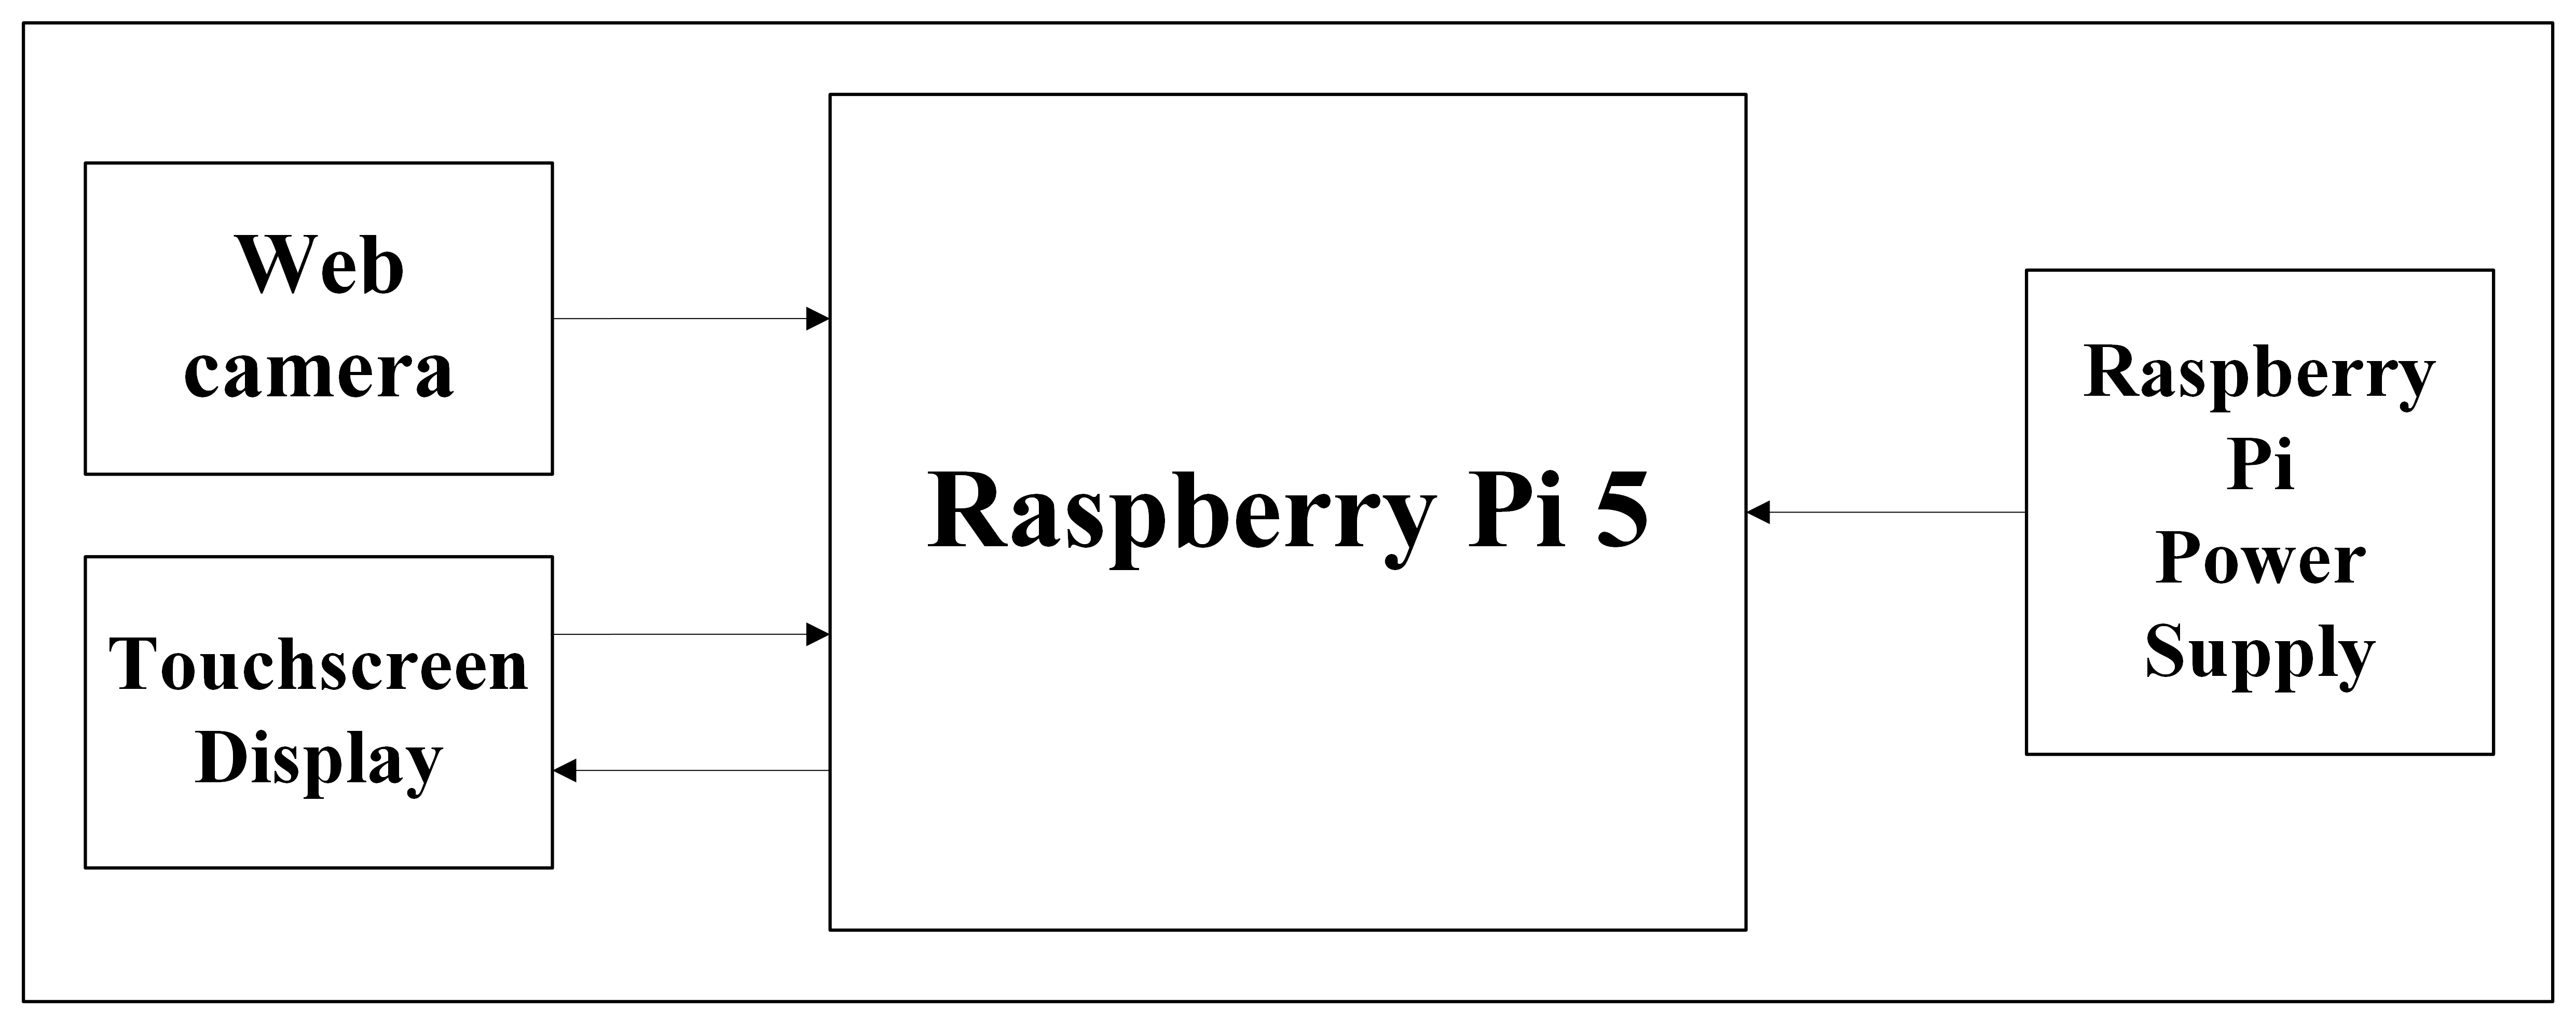
\includegraphics[width=3in]{blockdiag.png}}
                \vspace{-0.3cm}
                \caption{System block diagram.} 
                \label{blockdiagram}
            \end{figure} 
            \vspace{-0.4cm}
            \indent The system block diagram is shown in Figure 
            \ref{blockdiagram}. The system is composed of a 
            Raspberry Pi 5, a web camera, and a 
            touchscreen monitor. The Raspberry Pi 5 is the main 
            processing unit of the system. The web camera is 
            used for capturing images of handwritten lecture notes. 
            The touchscreen monitor is used for displaying the 
            generated questions. The system is enclosed in a box 
            with proper illumination for the facilitation of the 
            processes.
        \vspace{0.2cm}
        \subsubsection{Experimental Setup}
            \hfill \\
            \vspace{-0.6cm}
            \begin{figure}[H]
                \centerline{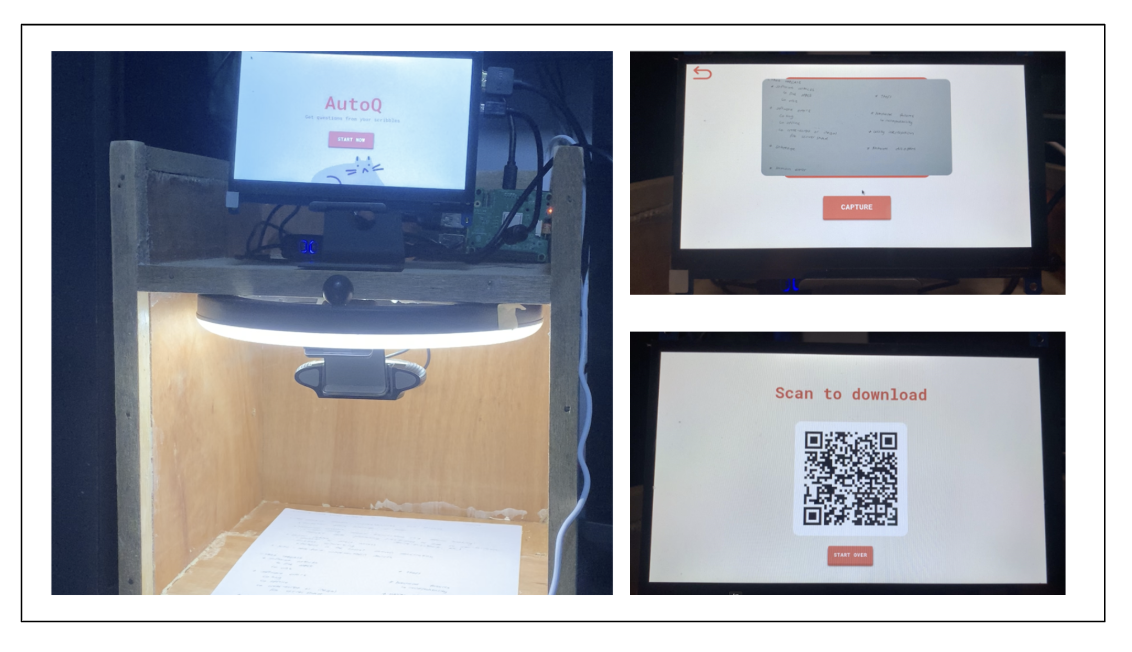
\includegraphics[width=3in]{experimental.png}}
                \vspace{-0.3cm}
                \caption{Experimental setup.} 
                \label{experimental}
            \end{figure} 
            \vspace{-0.3cm}
            \indent The experimental setup is shown in 
            Figure \ref{experimental}. The system is enclosed in a
            constructed wooden box with proper illumination. The
            Raspberry Pi 5 is connected to the web camera and the
            touchscreen monitor. The web camera is used for capturing
            images of handwritten lecture notes. The touchscreen
            monitor is used for guiding the user in the system
            processes.
    \subsection{Software Development}
        \subsubsection{System Flowchart}
            \hfill \\
            \begin{figure}[H]
                \centerline{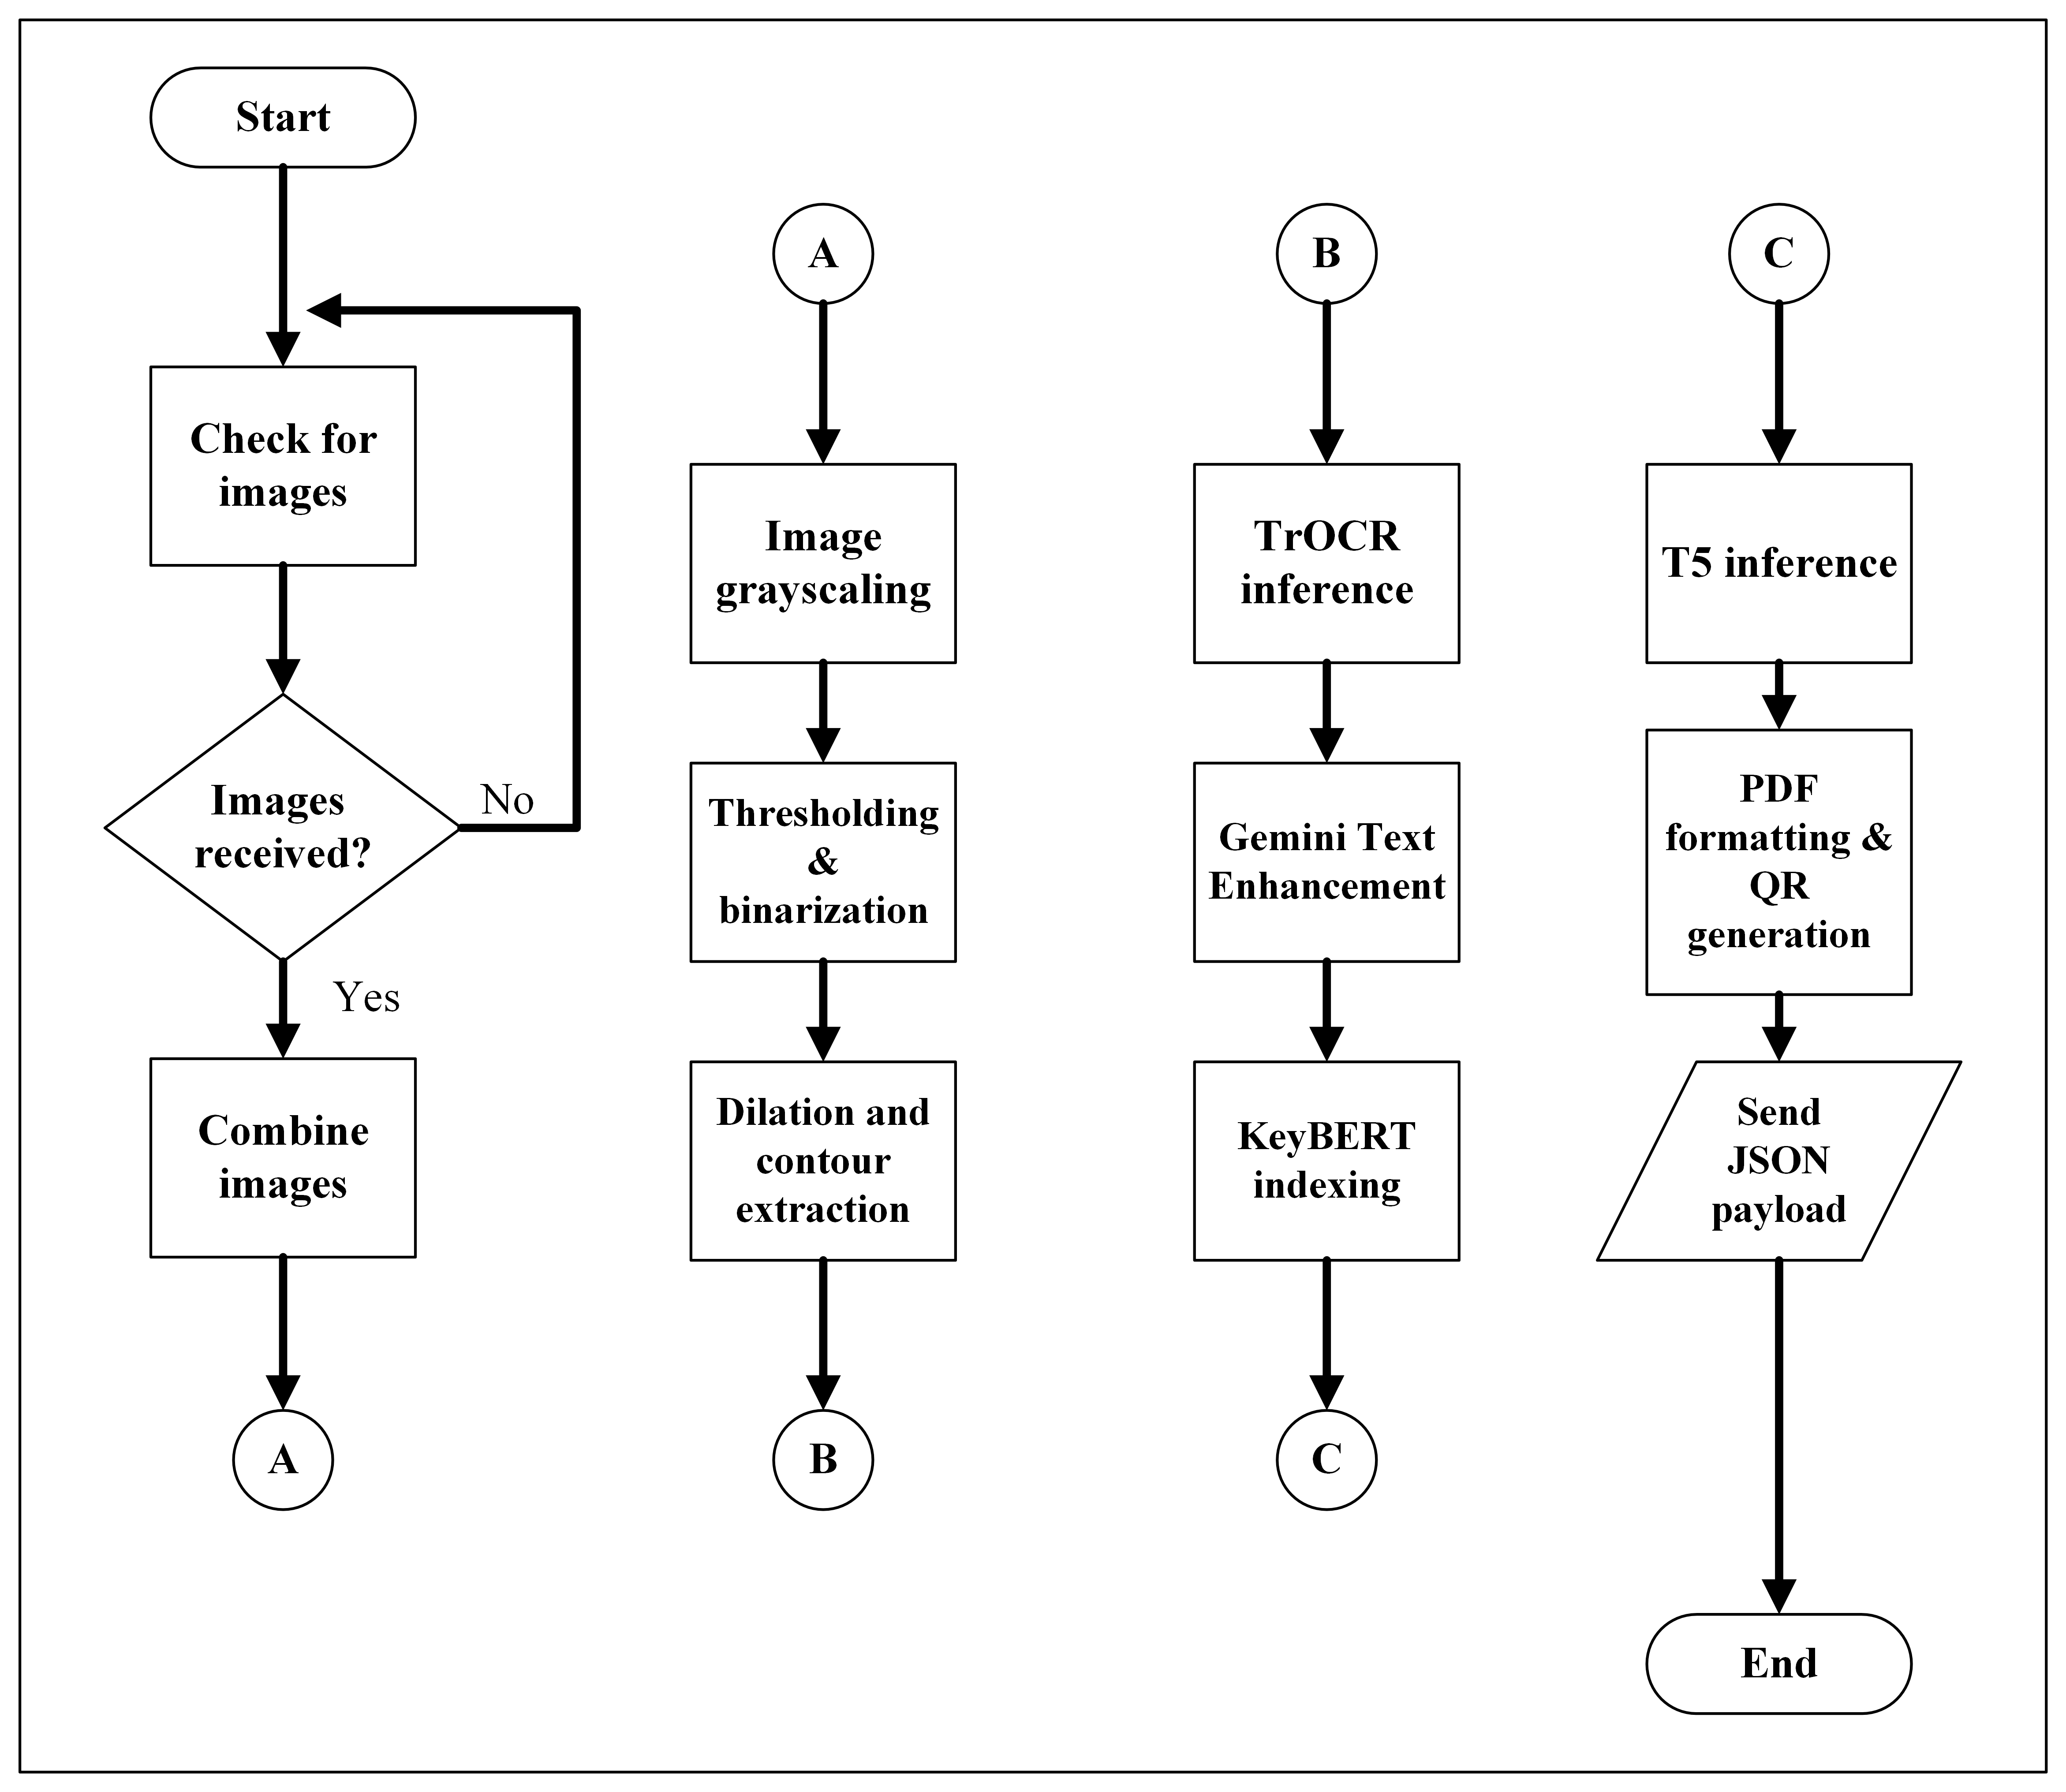
\includegraphics[width=3in]{flowchart.png}}
                \vspace{-0.4cm}
                \caption{System flowchart.} 
                \label{flowchart}
            \end{figure}
            \indent The system flowchart is shown in 
           Figure \ref{flowchart}. The system 
           starts with the collection and expectation of 
           the image captures of the top and bottom halves 
           of the notes. The image captures are then
           combined and undergone a series of image 
           transformations that extracts the text lines. 
           These text lines are inputted to the TrOCR for 
           inferencing and the extracted text is then
           inputted to the T5 for AQG. The generated
           questions are formatted to a portable document
              format (PDF) and uploaded to Google Drive 
            where a QR is generated for the user to download 
            the PDF on their device. JSON payload is then sent 
            to the front end of the system for the 
            notification on the touchscreen display.
        \vspace{0.4cm}
        \subsubsection{T5 AQG}
            \hfill \\
            \vspace{-0.5cm}
            \begin{figure}[H]
                \centerline{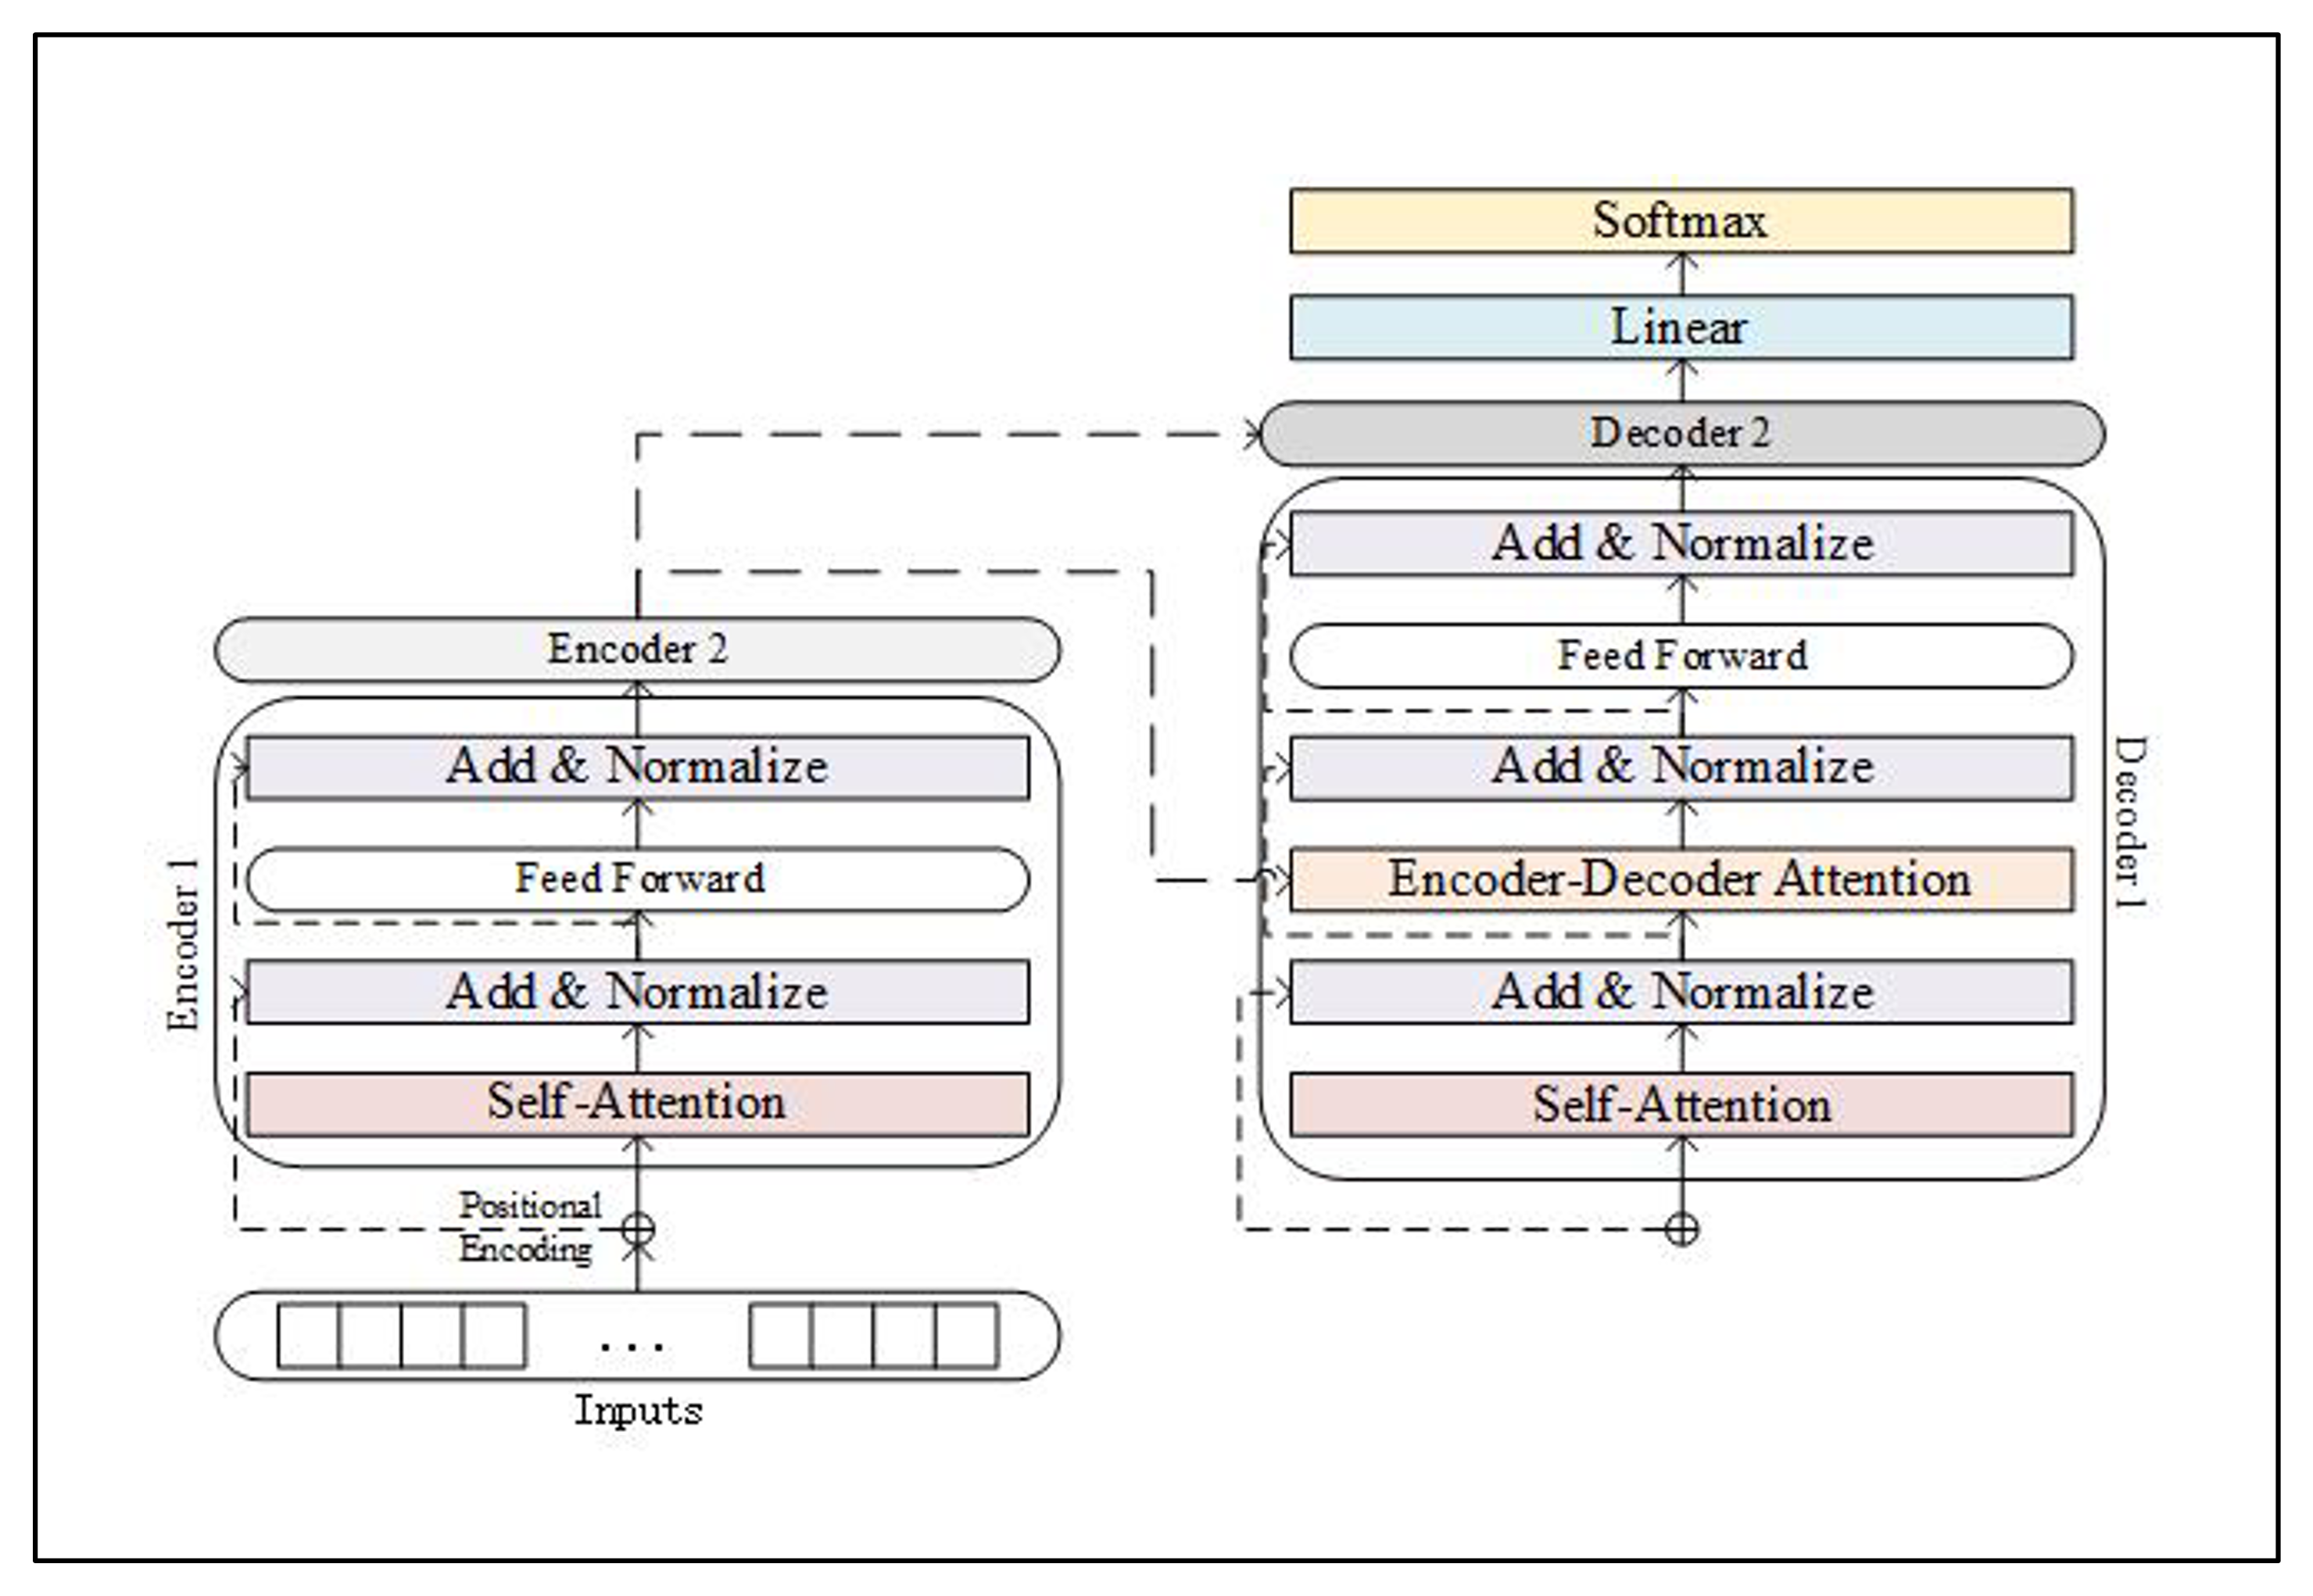
\includegraphics[width=3in]{t5arch.png}}
                \vspace{-0.4cm}
                \caption{T5 model architecture.} 
                \label{t5architecture}
            \end{figure}
            \vspace{-0.4cm}
            \indent Figure \ref{t5architecture} shows the 
            layers and components of the T5 model. 
            The important aspect from this is that T5 
            contains a final output layer that allows 
            for fine-tuning. \\ 
            \indent In this research, T5 was fine-tuned 
            to the SQuADv1.1 dataset. The input features 
            considered were the context and the chosen 
            answer phrase/keyword. The output feature
            was the question generated from the context
            and the chosen answer phrase/keyword. 
            
    \subsection{Data Gathering}
        \hfill \\
        \vspace{-1cm}
        \begin{figure}[H]
            \centerline{\includegraphics[width=3in]{datacollection.png}}
            \vspace{-0.3cm}
            \caption{Sample captured notes (with processed version on right).} 
            \label{datacollection}
        \end{figure} 
        \vspace{-0.3cm} 
        \indent A sample capture from the procured testing dataset 
        is shown in Figure \ref{datacollection}. 
        A total of 70 handwritten lecture notes were collected
        from an undergraduate class on computer networking and 
        cybersecurity. A total of 1800 text lines were extracted by the 
        system. These text lines were manually transcribed for reference.
        \\
        \indent From the top five keywords extracted from the handwritten notes
        (MAC, ethernet, address, data, frame), 
        a class of 27 students in the same course 
        were asked to generate questions from those top keywords. A 
        context was given to the students as a summary from the 
        notes. As such, 135 questions were collected for the comparison 
        between the model-generated questions versus the ones 
        from students.

    \subsection{Testing and Evaluation}

\section{Results and Discussion}
\section{Conclusion and Recommendations}

\section*{Acknowledgment}

The preferred spelling of the word ``acknowledgment'' in America is without 
an ``e'' after the ``g''. Avoid the stilted expression ``one of us (R. B. 
G.) thanks $\ldots$''. Instead, try ``R. B. G. thanks$\ldots$''. Put sponsor 
acknowledgments in the unnumbered footnote on the first page.

\section*{References}

Please number citations consecutively within brackets \cite{b1}. The 
sentence punctuation follows the bracket \cite{b2}. Refer simply to the reference 
number, as in \cite{b3}---do not use ``Ref. \cite{b3}'' or ``reference \cite{b3}'' except at 
the beginning of a sentence: ``Reference \cite{b3} was the first $\ldots$''

Number footnotes separately in superscripts. Place the actual footnote at 
the bottom of the column in which it was cited. Do not put footnotes in the 
abstract or reference list. Use letters for table footnotes.

Unless there are six authors or more give all authors' names; do not use 
``et al.''. Papers that have not been published, even if they have been 
submitted for publication, should be cited as ``unpublished'' \cite{b4}. Papers 
that have been accepted for publication should be cited as ``in press'' \cite{b5}. 
Capitalize only the first word in a paper title, except for proper nouns and 
element symbols.

For papers published in translation journals, please give the English 
citation first, followed by the original foreign-language citation \cite{b6}.

\end{document}
